\documentclass[conference]{IEEEtran}
% ============================================================
% LINGUAFORCE: Benchmarking Agentive Force of Discourse
% Release v1 -- IEEE conference format (11 pages)
%
% TODO before submission:
%  - Fill in real author names / affiliations
%  - One human agreement study on a subsample (LLM annotation is used now)
%  - Done: 15-type (T2) labels on the full release + supervised baseline (RoBERTa-base)
% ============================================================
\usepackage{cite}
\usepackage{amsmath,amssymb}
\usepackage{graphicx}
\usepackage{textcomp}
\usepackage{booktabs}
\usepackage{multirow}
\usepackage{array}
\usepackage{xcolor}
\usepackage{tikz}
\usetikzlibrary{arrows.meta,positioning,calc}
\usepackage[breaklinks=true]{hyperref}

% --- page-limit tightening ---
\setlength{\textfloatsep}{6pt plus 1pt minus 1pt}
\setlength{\floatsep}{6pt plus 1pt minus 2pt}
\setlength{\intextsep}{6pt plus 1pt minus 1pt}
\setlength{\dbltextfloatsep}{7pt plus 1pt minus 1pt}
\setlength{\dblfloatsep}{7pt plus 1pt minus 2pt}


\newcommand{\AFD}{Agentive Force of Discourse}

\newcommand{\afd}{agentive force of discourse}

\newcommand{\LNGF}{LINGUAFORCE}

\begin{document}

\title{\LNGF{}: Benchmarking \AFD{} in Dialogues via\\ Unified Psychological Dimensions}

\author{\IEEEauthorblockN{First Author, Second Author, Third Author}
\IEEEauthorblockA{\textit{School of Computer Science, Example University}\\
Example City, Country\\
\{first, second, third\}@example.edu}}

\maketitle

\begin{abstract}
Discourse that drives, guides, or restricts a listener's behavior---orders,
threats, inducements, guilt-tripping, peer pressure, gaslighting, and verbal
abuse---shares a common perlocutionary mechanism, yet existing benchmarks
study each strategy in isolation with incompatible labels and scales. We
propose \LNGF{}, a unified benchmark for the \afd{} in real-world multi-turn
dialogues, built on a three-layer framework: (i) a strategy taxonomy of four
families and fifteen types integrating compliance-gaining and speech-act
theory; (ii) seven universal psychological dimensions grounded in pragmatics
and persuasion research, which specialize to the obligation, constraint,
value-judgement, and toxicity channels in the present annotation scheme; and
(iii) a linguistic-realization layer linking dimensions to surface cues.
We release 3{,}432 re-annotated dialogues with intensity and seven-dimension
labels; reliability is verified through consistency with existing labels
and a two-annotator agreement study. The benchmark is designed to support
both detection and interpretability, since each prediction can be traced
back to a structured pressure profile. We define three benchmark tasks, a
two-stage dimension-aware pipeline, and cross-domain evaluation on
MentalManip, MultiManip, TalkDown, and ToxicChat, supporting zero-shot
recognition of unseen manipulation types.
\end{abstract}


\begin{IEEEkeywords}
Agentive force, perlocutionary pressure, computational social science,
psycholinguistic framework, large language models, manipulation detection.
\end{IEEEkeywords}
\section{Introduction}
Language does more than describe the world: utterances routinely act on
their listeners, driving, guiding, or restricting behavior. This
perlocutionary pressure appears across a broad range of everyday
strategies---a polite request that trades on reciprocity, an offer that
reframes a decision, an authority figure's direct command, a threat or
warning, social proof and conformity pressure, an emotional appeal, and
covert tactics such as gaslighting. These strategies differ in surface
form and intent, yet they share a common function: they operate on the
listener's decision space, expanding or constraining the options that
appear available. This listener-directed capacity is termed the
\emph{\afd{}}.

Current NLP research fragments this range across disconnected
communities. Toxicity detection targets explicit aggression but misses polite
or altruistic manipulation~\cite{toxicchat2023,talkdown2023}. Persuasion
technique detection focuses on news articles and rhetorical
framing~\cite{piskorski2023}. Psychological-manipulation datasets cover a
narrow subset of covert strategies such as gaslighting and intimidation and
rarely include benign or transparent requests as controls~\cite{mentalmanip,
multimanip,reament}. Compliance-gaining research in communication studies
provides rich taxonomies of persuasive strategies~\cite{marwell1967,
wiseman1981,cialdini1984} but has not been operationalized as a unified NLP
benchmark with continuous, comparable measurements. Taken together, these
gaps leave open three questions that matter for both science and safety:
(i)~what common structure underlies strategies as different as a polite
request, a threat, and gaslighting; (ii)~can a single measurement scale make
them comparable; and (iii)~can a model trained on a unified pressure space
recognize manipulation forms it has never seen?



Prior work studies many individual forms of influence, but the gap is not
only taxonomic: without a shared scale, it is hard to tell whether two
different strategies are genuinely comparable or merely labeled alike by
convention. It remains unclear whether a common set of psychological
dimensions can measure pressure across transparent, exchange,
social-normative, and covert strategies.

To address this focused gap, we introduce \LNGF{}, a benchmark for the
\afd{} in real-world multi-turn dialogues. The central question is whether
the strategy structure of agentive force can be represented by a shared set
of measurable dimensions. Generalization to strategies absent from the
training data is treated as a consequence to test, rather than as a second
definition of the phenomenon. The paper proceeds in four steps: related work
establishes the theoretical boundary; the framework defines the strategy and
dimension layers; the dataset section describes construction and validation;
and the experiments test measurement, structure, and transfer. Our
contributions are threefold:
\begin{enumerate}
\item \textbf{A unified three-layer framework.} We integrate
compliance-gaining theory, speech-act theory, and persuasion-technique
taxonomies into a strategy taxonomy of four families and fifteen types,
a universal inventory of seven psychological dimensions,
and a linguistic-realization layer that links each dimension
to observable surface cues. The framework specializes to the obligation,
constraint, value-judgement, and toxicity channels within the same unified
annotation scheme as consistency anchors.
\item \textbf{A new dataset and benchmark.} We construct \LNGF{}, a
3{,}432-dialogue dataset with dialogue-level annotations of intensity and
seven psychological dimensions; annotation reliability is verified through
consistency with existing labels on shared dialogues.
\item \textbf{An experimental protocol.} We define three tasks (detection,
type recognition, and intensity prediction), a two-stage dimension-aware
pipeline, a zero-shot evaluation against a direct baseline, and research
questions on dimension structure and zero-shot generalization to unseen
manipulation types.
\end{enumerate}
\section{Related Work}
This section establishes the conceptual basis for treating agentive force as
listener-directed action rather than as a synonym for toxicity or
manipulation. It then identifies the specific gap addressed by the benchmark:
existing resources lack a common strategy inventory and a comparable pressure
measurement.
\subsection{Datasets of Manipulation and Persuasion}
Communication research has long studied compliance-gaining: Marwell and
Schmitt~\cite{marwell1967} extracted sixteen strategies and
Wiseman and Schenck-Hamlin~\cite{wiseman1981} fourteen, later organized by
Cialdini~\cite{cialdini1984} into reciprocity, commitment, social proof,
authority, liking, and scarcity. In NLP, SemEval-2023 Task~3 detects
persuasion techniques in online news~\cite{piskorski2023}, and recent
datasets target covert manipulation in dialogues: MentalManip,
MultiManip~\cite{mentalmanip,multimanip}, and ReaMent~\cite{reament}. These
resources are valuable but narrow: they either target monological news text
or focus on covert and pathological strategies, omit benign and transparent
controls (requests, advice, rational persuasion), and use incompatible label
spaces. Toxicity detection~\cite{toxicchat2023}, condescension
detection~\cite{talkdown2023}, and microaggression work~\cite{breitfeller2019}
cover the abusive end of this range but treat hostility as the phenomenon
rather than as a channel of listener-directed pressure. \LNGF{} covers the
negative, listener-restricting portion of this range: pressure that drives or
constrains a target in the speaker's preferred direction. Transparent
requests, advice, and rational persuasion are retained as controls and
boundary cases, not claimed as equivalent to covert abuse. Positive influence
such as praise or encouragement may also change a listener's decision space,
but it is outside the present release and is reserved for a future extension.

\subsection{Speech Acts and Agentive Force}
Speech-act theory distinguishes what an utterance says from what it does in
interaction~\cite{austin1962,searle1969}. This distinction provides the
starting point for \afd{}: the object of measurement is not whether a
sentence contains an aggressive word, but whether it is used to alter a
listener's available or acceptable actions. The term is also distinct from
the speaker-oriented notion of linguistic agency in anthropology~\cite{ahearn2001};
our unit is the pressure exerted on the listener's decision space.

\subsection{Normative Influence and Moral Foundations}
Normative influence invokes duties, roles, morality, authority, or group
identity to steer behavior. Moral foundations theory~\cite{graham2009} (care,
fairness, loyalty, authority, sanctity, liberty) grounds our normative
family~C: C1 (moral appeal) typically loads on care and loyalty, while C4
(authority) loads on authority and liberty, sharpening the boundary between
normative pressure and pure threats ($D_2$).

\subsection{Agentive Force in LLM Safety Evaluation}
Beyond detection, \afd{} matters for LLM safety. Current evaluations measure
explicit harms such as toxicity, bias, and refusal correctness but rarely
score manipulative \emph{styles}---guilt-heavy advice, authority-laden
justifications, false-dilemma framings---even though they can steer users
toward harmful decisions in health, finance, and politics. \LNGF{}'s
seven-dimension profile provides a continuous, interpretable measurement
applicable to generated text (e.g., scoring $D_2$ or $D_3$ with the same
rubric used for human dialogue), making the benchmark a dual-purpose
instrument: a detection benchmark for human conversation and a safety rubric
for auditing model behavior. In linguistic anthropology,
Ahearn~\cite{ahearn2001} uses ``linguistic agency'' for the speaker's
socioculturally mediated capacity to act; to avoid conflation with our
listener-directed notion, we use \emph{\afd{}} (equivalently, perlocutionary
pressure) throughout.

\section{Framework: A Unified Account of \afd}
\label{sec:framework}
This section gives the paper's main conceptual answer: agentive force is a
listener-directed, scalar pressure effect with a functional strategy layer,
a psychological measurement layer, and a linguistic-cue layer. The three
layers separate what a speaker does, how strongly it acts on the listener,
and which observable signals support the judgment.
\subsection{Definition and Inclusion Criterion}
We define the \emph{\afd{}} of an utterance or dialogue as its perlocutionary
capacity to drive, guide, or restrict a listener's behavior and decision
space: the pressure an utterance exerts to shift the listener's acceptable
action set toward the speaker's preferred subset, along one or more of seven
channels. Three properties matter. \emph{Success is not required}:
perlocutionary force exists even when the listener resists. \emph{Force is
compositional}: an utterance can combine channels (e.g., guilt plus social
proof). \emph{Force is scalar}: strategies differ in intensity, not only in
kind.

A discourse has \emph{\afd{}} iff it (i)~targets a recognizable action or
decision of the listener and (ii)~aims to drive or restrict behavior through
pressure, inducement, norm invocation, emotional leverage, deception, or
hostility. The taxonomy below operationalizes these mechanisms; it is not a
claim that the fifteen listed types exhaust every possible realization. Pure
information and
emotional venting are excluded and serve as negative examples, making the
negative class meaningful---a common weakness in manipulation benchmarks.

\subsection{Three-Layer Architecture}
Figure~\ref{fig:framework} shows the architecture. Layer~1 is the strategy
inventory: what the speaker does. Layer~2 is the pressure profile: how much
force is applied along seven psychological dimensions. Layer~3 is the cue
map: which observable words, constructions, and discourse patterns reveal
that force. Layer~1 contains fifteen types in four families, while Layers~2
and~3 support comparison beyond any one type list.
Jointly annotating the three layers lets models reason at the intended
abstraction level and enables error analysis impossible with binary labels
alone.

\begin{figure*}[t]
\centering
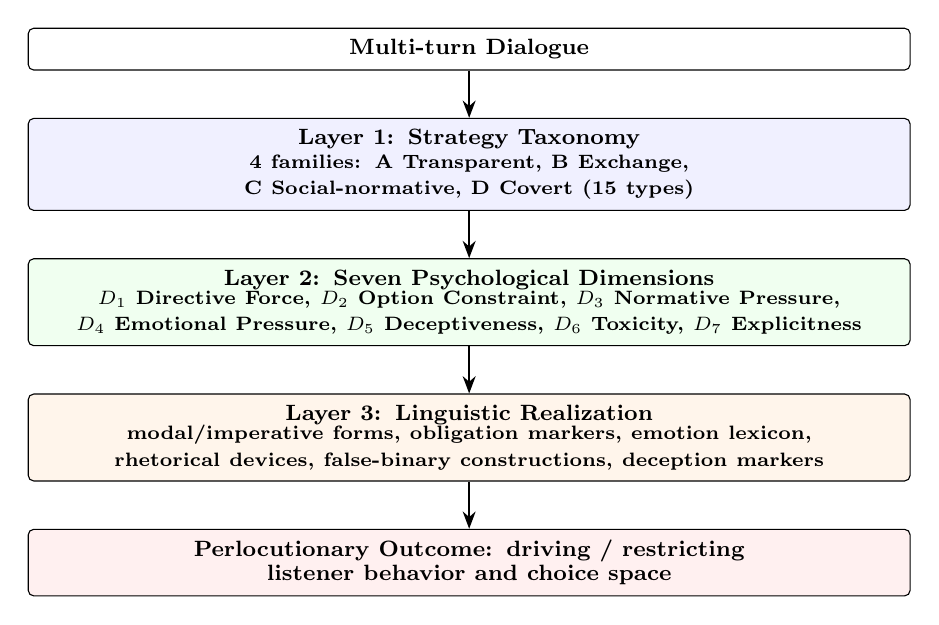
\begin{tikzpicture}[
  lbl/.style={draw, rounded corners=2pt, align=center, inner sep=4pt, text width=10.6cm,
              font=\footnotesize\bfseries, minimum width=11.2cm},
  arr/.style={-{Stealth[length=2.2mm]}, semithick}
]

\node[lbl] (d) {Multi-turn Dialogue};

\node[lbl, below=6mm of d, fill=blue!6] (l1) {Layer 1: Strategy Taxonomy\\[-1pt]
\scriptsize 4 families: A Transparent, B Exchange, C Social-normative, D Covert (15 types)};

\node[lbl, below=6mm of l1, fill=green!6] (l2) {Layer 2: Seven Psychological Dimensions\\[-1pt]
\scriptsize $D_1$ Directive Force, $D_2$ Option Constraint, $D_3$ Normative Pressure,\\ $D_4$ Emotional Pressure, $D_5$ Deceptiveness, $D_6$ Toxicity, $D_7$ Explicitness};

\node[lbl, below=6mm of l2, fill=orange!8] (l3) {Layer 3: Linguistic Realization\\[-1pt]
\scriptsize modal/imperative forms, obligation markers, emotion lexicon,\\ rhetorical devices, false-binary constructions, deception markers};

\node[lbl, below=6mm of l3, fill=red!6] (o) {Perlocutionary Outcome: driving / restricting\\[-1pt] listener behavior and choice space};
\draw[arr] (d) -- (l1);
\draw[arr] (l1) -- (l2);
\draw[arr] (l2) -- (l3);
\draw[arr] (l3) -- (o);
\end{tikzpicture}
\caption{Three-layer architecture of \LNGF. The strategy taxonomy defines
what the speaker does, the psychological dimensions measure how much pressure
is applied, and the linguistic-realization layer links both to surface cues.
Normative pressure is expected to be high when the speaker invokes duty,
morality, or social roles, while explicitness depends on whether that pressure
is stated directly or indirectly.}
\label{fig:framework}
\end{figure*}

\subsection{Strategy Taxonomy}
\label{sec:taxonomy}
Table~\ref{tab:taxonomy} presents the taxonomy. The four families organize
the current negative-force scope by the dominant mechanism: A (transparent)
contains direct, openly stated requests, advice, orders, and reasoning and
provides the behavioral baseline; B (exchange) motivates through anticipated
benefit or harm; C (social-normative) invokes duties, roles, morality,
authority, reciprocity, or group conformity; D (covert) relies on emotional
exploitation, deception, false dilemmas, or hostility. These families are
descriptive organizing units, not mutually exclusive psychological causes,
and one dialogue may receive multiple type labels. The final column in
Table~\ref{tab:taxonomy} records the dominant mechanism used by each type;
these mechanisms are descriptive and do not imply mutually exclusive causes.
\begin{table*}[t]
\centering
\caption{Strategy taxonomy of \LNGF: four families and fifteen types.
The mechanism column records the dominant pressure channel for each type.}
\label{tab:taxonomy}
\scriptsize
\begin{tabular}{@{}p{1.9cm}p{2.5cm}p{6.6cm}p{2.0cm}p{2.0cm}@{}}
\toprule
\textbf{Family} & \textbf{Type} & \textbf{Description and example} & \textbf{Mechanism} & \textbf{Role}\\
\midrule
\multirow{3}{*}{\parbox{1.7cm}{A. Transparent}}
 & A1 Request/Advice & Low-pressure, intention-transparent proposal. \emph{``Could you revise this report by Friday?''} & --- & benign control\\
 & A2 Directive/Order & Direct instruction with expected compliance. \emph{``Send the report before you leave.''} & --- & transparent pressure\\
 & A3 Rational Persuasion & Argument, evidence, expert opinion. \emph{``The data show 30\% lower cost; adopt it.''} & --- & reasoned pressure\\
\multirow{2}{*}{\parbox{1.7cm}{B. Exchange}}
 & B1 Promise/Inducement & Benefit-driven motivation. \emph{``Help me this once and I will return the favor.''} & --- & incentive pressure\\
 & B2 Threat/Warning & Harm-driven motivation. \emph{``If you do not sign, you will face consequences.''} & constraint & explicit constraint\\
\multirow{6}{*}{\parbox{1.7cm}{C. Social-normative}}
 & C1 Moral Appeal/Guilt & Appeals to conscience or moral duty. \emph{``A dutiful son would never let his mother suffer.''} & normative & normative core\\
 & C2 Obligation/Duty & Invokes role responsibilities. \emph{``You are the team leader; it is your duty.''} & normative & duty pressure\\
 & C3 Value Judgement/Shaming & Moral labeling of the target. \emph{``You are so selfish; you never think of others.''} & normative & moral attack\\
 & C4 Authority & Appeals to status, rank, seniority. \emph{``The boss decided; why keep arguing?''} & --- & hierarchical pressure\\
 & C5 Conformity/Social Proof & Appeals to group norms. \emph{``Everyone is doing it; why are you special?''} & --- & peer pressure\\
 & C6 Reciprocity/Debt & Invokes past favors. \emph{``I helped you last time; do not refuse this.''} & --- & debt pressure\\
\multirow{4}{*}{\parbox{1.7cm}{D. Covert}}
 & D1 Emotional Manipulation & Feigned weakness, pity, or fear to steer behavior. \emph{``If you leave too, I do not know what to do.''} & --- & affective leverage\\
 & D2 Deception/Gaslighting & Distorts facts or memory. \emph{``I never said that; you misremember.''} & --- & epistemic attack\\
 & D3 Logical Trap/False Dilemma & Shrinks the option space. \emph{``Either you follow me or we are done.''} & constraint & option elimination\\
 & D4 Verbal Abuse/Toxicity & Explicit hostility and disparagement. \emph{``You are useless; you cannot even do this.''} & hostility & hostile pressure\\
\bottomrule
\end{tabular}
\end{table*}

\subsection{Universal Psychological Dimensions}
\label{sec:dims}
Table~\ref{tab:dims} defines seven dimensions on a continuous 0--1 scale
(with a companion four-level discrete label), at both turn and dialogue
level. Within the present negative-force scope, every listed strategy maps to
at least one dimension. The seven dimensions are therefore a proposed
measurement basis, not a claim of psychological completeness; their
usefulness must be judged by reliability, discriminative value, and transfer.
The dimensions are defined directly from the mechanisms represented in the
taxonomy, so every dialogue can be embedded in the same seven-dimensional
space and evaluated with the same rubric.

\begin{table}[t]
\centering
\caption{Seven psychological dimensions used to measure negative agentive
force.}
\label{tab:dims}
\footnotesize
\begin{tabular}{@{}p{1.15cm}p{4.4cm}p{2.5cm}@{}}
\toprule
\textbf{Dim.} & \textbf{Definition} & \textbf{Role}\\
\midrule
$D_1$ Directive Force & Strength with which the utterance drives a target action & generalization (new)\\
$D_2$ Option Constraint & Degree to which the listener's options are narrowed & choice restriction\\
$D_3$ Normative Pressure & Pressure via duty, morality, norms, roles & social steering\\
$D_4$ Emotional Pressure & Use of guilt, shame, fear, pity as leverage & new\\
$D_5$ Deceptiveness & Degree of factual or epistemic distortion & new\\
$D_6$ Toxicity & Explicit hostility and abuse & hostile pressure\\
$D_7$ Explicitness & Transparency vs.\ indirectness of the pressure & new\\
\bottomrule
\end{tabular}
\end{table}

The reused dialogues therefore double as a validation set: morally coercive
dialogues should receive high $D_3$ and low-to-moderate $D_7$. We also expect
each family to load on a small set of dimensions---$D_3$ for family~C,
$D_2$/$D_4$ for B, $D_5$/$D_6$ for D---examined via per-family profiles and
clustering (Section~\ref{sec:dataset}) as quality checks and descriptive
evidence.
\subsection{Linguistic Realization Layer}
Table~\ref{tab:cues} links each dimension to typical surface realizations.
The layer makes annotation operational (annotators justify scores from a cue
checklist, improving agreement), supports error analysis (failures trace to
missing cues, cue ambiguity, or long-range context), and connects \LNGF{} to
explainability: upstream-parser dimension scores (Section~\ref{sec:exp}) are
directly verbalizable as cue-based rationales.

\begin{table}[t]
\centering
\caption{Illustrative surface cues per dimension. Cues are indicative, not
sufficient: a cue only counts when the discourse targets the listener's
behavior.}
\label{tab:cues}
\scriptsize
\begin{tabular}{@{}p{1.35cm}p{6.7cm}@{}}
\toprule
\textbf{Dim.} & \textbf{Typical cues}\\
\midrule
$D_1$ & imperative and hortative forms; modal ``must/should/have to''; performative requests\\
$D_2$ & ``either/or'', ultimatums, no-alternative framings, threats of consequence\\
$D_3$ & duty and role nouns, moral adjectives, normative ``ought''; appeal to what ``a good X'' would do\\
$D_4$ & emotion lexicon (guilt, shame, fear, pity), emotional blackmail, self-deprecation\\
$D_5$ & fact distortions, memory disputes, gaslighting patterns, manufactured consensus\\
$D_6$ & insults, disparagement, profanity, dehumanizing labels\\
$D_7$ & direct address and explicit request vs.\ hints, presuppositions, innuendo\\
\bottomrule
\end{tabular}
\end{table}

\subsection{A Worked Annotation Example}
Table~\ref{tab:example} shows a worked annotation. The dialogue mixes moral
appeal (C1) and obligation (C2), hence receives a multi-label type
annotation; intensity is high and the profile is dominated by $D_3$ with
secondary $D_1$. The example illustrates why the task is hard: the language
is polite (no $D_6$) and the pressure implicit (low $D_7$)---the pattern that
defeats lexical toxicity classifiers.

\begin{table*}[t]
\centering
\caption{A worked annotation example. S = speaker turn; L = listener turn.
Type, intensity, and the seven dimension scores are annotated per turn and
aggregated at dialogue level.}
\label{tab:example}
\scriptsize
\begin{tabular}{@{}p{0.8cm}p{5.8cm}p{5.2cm}p{3.2cm}@{}}
\toprule
\textbf{Turn} & \textbf{Utterance} & \textbf{Type (multi-label)} & \textbf{Dimension profile}\\
\midrule
S1 & ``A dutiful son would never let his mother live alone; you are not that kind of person, are you?'' & C1 Moral Appeal; C3 Value Judgement & $D_3{=}0.9$, $D_1{=}0.7$, $D_4{=}0.6$, $D_7{=}0.4$\\
L1 & ``I know, but my job requires me to move...'' & --- (defensive) & $D_1{=}0.2$\\
S2 & ``Your mother sacrificed everything for you; it is your turn to repay her.'' & C2 Obligation; C6 Reciprocity & $D_3{=}0.9$, $D_2{=}0.5$, $D_1{=}0.8$\\
\midrule
\multicolumn{3}{@{}l}{\textbf{Dialogue-level}} & \textbf{Intensity 4/5; T1 positive; C1+C2+C3+C6}\\
\bottomrule
\end{tabular}
\end{table*}


\subsection{Dimension Structure and Interdependence}
The dimensions are not assumed independent; their correlation structure is
an empirical object that we state explicitly so it can be falsified.
(i)~$D_1$ should correlate with $D_2$ (the harder the push, the narrower the
options), with transparent A1 as the predicted exception. (ii)~$D_3$ and
$D_4$ should co-occur in family~C (guilt and moral appeal are emotionally
loaded) but separate in family~B (threats are affectively cold).
(iii)~$D_5$ should be roughly orthogonal to the others---gaslighting occurs
in both polite and hostile registers---so a strong correlation with $D_6$ or
$D_7$ would indicate annotation bias. (iv)~$D_7$ should correlate negatively
with $D_5$: covert strategies are typically indirect. The statistical
analysis (Section~\ref{sec:dataset}) tests these via correlation matrices
and per-family profiles; deviations are reported and used to revise the
guideline rather than discarded.


\section{Dataset Construction and Analysis}
\label{sec:dataset}
\subsection{Design Principles}
This section explains what evidence is needed to make the definition
measurable: coverage of the intended negative-force scope, comparable labels
for every dialogue, and hard negatives that separate pressure from mere
toxicity or ordinary requests.
Four principles guide construction. (i)~\emph{Real-world multi-turn
dialogues}: authentic interaction rather than scripted text, which lacks the
fragmentation and pragmatic embedding of real conversation.
(ii)~\emph{Scope coverage}: negative-force and non-force dialogue across
the 0--5 range, so benign controls prevent degenerate models that classify
any request as manipulation. (iii)~\emph{Comparable measurement}: every
instance receives the same seven-dimension annotation on one scale.
(iv)~\emph{Hard negatives}: polite coercion, sarcastic requests, and
superficially kind manipulation stress-test lexical shortcuts.

\subsection{Sources and Sampling}
\LNGF{} re-annotates an existing, de-identified corpus of everyday
multi-turn dialogues, retaining its source binary pressure and 0--5
intensity labels for validation. The full release is the 3{,}432-
dialogue training partition; a disjoint 634-dialogue held-out partition is
released as a consistency-check set (Section~\ref{sec:firstrelease}) and its
statistics are reported alongside. Dialogues are already de-identified, so
the negative class and the intensity tail arise naturally without new
collection.

\begin{table}[t]
\centering
\caption{Released \LNGF{} sets.}
\label{tab:dataset}
\footnotesize
\begin{tabular}{@{}lccc@{}}
\toprule
\textbf{Set} & \textbf{Dialogues} & \textbf{Coercive} & \textbf{Non-coercive}\\
\midrule
Full release & 3{,}432 & 1{,}862 (54.2\%) & 1{,}570 (45.8\%)\\
First-release held-out & 634 & 332 (52.4\%) & 302 (47.6\%)\\
\bottomrule
\end{tabular}
\end{table}




\subsection{Annotation Protocol}
The annotation protocol tests whether the abstract definition can be applied
consistently: first identify a listener-directed behavioral target, then the
mechanism, and only then its intensity and dimension profile. Annotation
follows a three-level decision tree: (1)~Does the discourse target
a listener action or decision? If no, it is a negative example. (2)~Which
strategies from Table~\ref{tab:taxonomy} are present? (multi-label; a
dialogue may combine, e.g., moral appeal and social proof). (3)~What are the
intensity and the seven dimension scores? Intensity is ordinal 0--5; each
dimension receives a continuous 0--1 score and a four-level discrete label
(None/Low/Moderate/High). In this release the annotation is produced by an
instruction-tuned LLM (Section~\ref{sec:exp}) that follows the decision tree
and emits a structured JSON profile for each dialogue at temperature~$0$ for
reproducibility. Reliability is validated through the consistency checks
against the existing labels in Section~\ref{sec:firstrelease} and through a
two-annotator agreement study on a stratified subsample
(Section~\ref{sec:qc}).

\subsection{Annotation Decision Tree and Negative Cases}
To keep the negative class principled, annotation follows the decision tree
in Figure~\ref{fig:tree}: the first question filters out ordinary
conversation, the second assigns strategy labels, and the third assigns
intensity and dimension scores. Negative examples are annotated at the same
granularity as positives so the dimension space covers the intended
negative-force range.
Typical negatives include pure information exchange, emotional venting with
no behavioral target, and information-seeking questions. Borderline cases
(e.g., advice that is also a subtle request) are resolved by the multi-label
rule: assign every applicable type and let dimension scores capture the
dominant channel.

\begin{figure}[t]
\centering
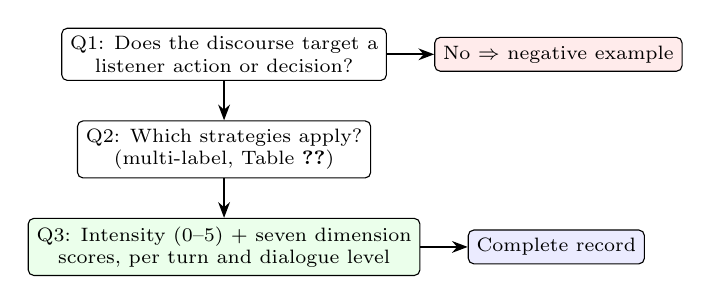
\begin{tikzpicture}[
  tn/.style={draw, rounded corners=2pt, align=center, font=\scriptsize, inner sep=3pt},
  arr/.style={-{Stealth[length=2mm]}, semithick}
]

\node[tn] (q1) {Q1: Does the discourse target a\\ listener action or decision?};

\node[tn, right=6mm of q1, fill=red!8] (no) {No $\Rightarrow$ negative example};

\node[tn, below=5mm of q1, xshift=0cm] (q2) {Q2: Which strategies apply?\\ (multi-label, Table~\ref{tab:taxonomy})};

\node[tn, below=5mm of q2, fill=green!8] (q3) {Q3: Intensity (0--5) + seven dimension\\ scores, per turn and dialogue level};

\node[tn, right=6mm of q3, fill=blue!8] (out) {Complete record};
\draw[arr] (q1) -- (no);
\draw[arr] (q1) -- (q2);
\draw[arr] (q2) -- (q3);
\draw[arr] (q3) -- (out);
\end{tikzpicture}
\caption{Three-question annotation decision tree.}
\label{fig:tree}
\end{figure}

\subsection{Quality Control and Consistency Validation}
\label{sec:qc}
The purpose of quality control is to establish that the proposed dimensions
are reproducible measurements rather than labels copied from a single binary
judgment. We therefore combine agreement evidence with consistency and
monotonicity checks against the source annotations.
Because annotation is LLM-produced rather than crowd-sourced, quality
control combines measurable consistency with the source corpus's gold
labels with a manual re-annotation check. We report, for every
dimension, its Spearman correlation with the source binary pressure label and the
0--5 intensity label, and the AUC for separating coercive from non-coercive
dialogues (Table~\ref{tab:full}); a dimension that fails
to track the gold labels is flagged as an unreliable anchor. We additionally
check that the predicted intensity is monotonic in the gold label
(Figures~\ref{fig:mono-full} and~\ref{fig:mono-full}) and that the inter-dimension
correlation matrix shows no pathological coupling
(Figures~\ref{fig:dim-corr-full} and~\ref{fig:dim-corr-full}). To probe reliability beyond label consistency, the first author
manually annotated a stratified subsample of 120 dialogues (balanced on
the gold binary label and spanning all intensity levels), following the
same annotation rubric as the automatic pipeline. Agreement with the
automatic profiles is high on overall agency strength
(Spearman $\rho{=}0.79$), and the primary pressure mechanism matches the
automatic profile's top two dimensions in 81.2\% of the 85
mechanism-bearing cases (excluding the explicitness meta-dimension
$D_7$, which marks directness rather than a specific pressure channel).
These results indicate that the seven-dimension profiles are
reproducible against independent human judgment.

To further probe reliability beyond the author's spot-check, we ran a
two-annotator agreement study on a stratified subsample of 150 dialogues
(balanced on the binary label), annotated independently under the same
rubric. Table~\ref{tab:iaa} reports inter-annotator agreement on the
discrete labels: the core intensity label reaches substantial agreement
(quadratic-weighted $\kappa{=}0.73$), as do normative pressure (0.78),
toxicity (0.76), and option constraint (0.66); binary presence and
explicitness reach moderate agreement (0.49), and deceptiveness is the
least reliable dimension (0.39), consistent with its subjective,
low-frequency nature. The continuous scores inherit the same ordering as
the discrete labels, so the reported agreement carries over to the
released scores.

\begin{table}[t]
\centering
\caption{Inter-annotator agreement on a stratified subsample ($n{=}150$;
two independent annotators, 149 fully labeled pairs). Binary uses
unweighted Cohen's $\kappa$; intensity and dimensions use
quadratic-weighted $\kappa$.}
\label{tab:iaa}
\footnotesize
\begin{tabular}{@{}lcc@{}}
\toprule
\textbf{Variable} & \textbf{Cohen's $\kappa$} & \textbf{Agreement level}\\
\midrule
binary (pressure present) & 0.49 & moderate\\
intensity (0--5) & 0.73 & substantial\\
$D_1$ directive force & 0.55 & moderate\\
$D_2$ option constraint & 0.66 & substantial\\
$D_3$ normative pressure & 0.78 & substantial\\
$D_4$ emotional pressure & 0.60 & substantial\\
$D_5$ deceptiveness & 0.39 & fair\\
$D_6$ toxicity & 0.76 & substantial\\
$D_7$ explicitness & 0.49 & moderate\\
\bottomrule
\end{tabular}
\end{table}



\subsection{Statistical Analyses}
The analyses below answer one question: do the dimensions behave like a
structured measurement of agentive force, rather than seven correlated
rephrasings of the same label? We report: (i)~per-dimension means and consistency with the gold labels
(Table~\ref{tab:full}); (ii)~the dimension correlation matrix, testing
whether $D_3$--$D_4$ co-occur while $D_5$ stays orthogonal
(Figure~\ref{fig:dim-corr-full}); (iii)~the
separation of coercive and non-coercive dialogues in the seven-dimensional
space (Figure~\ref{fig:box-full}); and (iv)~the
monotonicity of predicted intensity in the gold 0--5 label
(Figure~\ref{fig:mono-full}). These analyses also serve
as sanity checks against spurious lexical correlations, a failure mode
identified in prior manipulation datasets. Type-level analyses on the type-labeled split are reported in
Section~\ref{sec:results}.


\subsection{First Release and Consistency with Existing Labels}
\label{sec:firstrelease}
This subsection asks whether the new seven-dimensional profile recovers the
known ordering of negative agentive force before the full release is used.
Agreement with the source labels is necessary for validity, but by itself it
does not establish that the dimensions are useful or causally effective.
To validate the framework before scaling annotation, we release a first
consistency-check set: the 634-dialogue held-out split of the
underlying corpus, re-annotated under the unified seven-dimension
scheme. The set contains 332 coercive (52.4\%) and 302 non-coercive
dialogues, and gold intensity is distributed as
170/54/78/64/107/161 over levels 0--5, so hard negatives and the
high-intensity tail are both represented.

Table~\ref{tab:rq1} and Figures~\ref{fig:dim-gold-full}--\ref{fig:dim-corr-full}
report the consistency of the extracted profiles with the existing labels.
All seven dimensions correlate with the source binary pressure label and with the
0--5 intensity label; the strongest channels are option constraint ($D_2$), directive force
($D_1$), and emotional pressure ($D_4$), followed by explicitness
($D_7$) and normative pressure ($D_3$); this is consistent with
constraint being a core channel of
moral-pressure labels. Each dimension separates
coercive from non-coercive dialogues with AUC between 0.72 and 0.83. The
predicted intensity rises monotonically with the gold label
(Spearman $\rho{=}0.66$), and the inferred binary decision reaches AUC
0.83 and F1 0.80 at the best threshold, confirming that the unified
dimension space reproduces---and can in principle subsume---the prior
corpus's own measurement on the shared dialogues. A direct zero-shot judge
that bypasses the profile achieves AUC 0.78 and best F1 0.76 on the same
dialogues (Section~\ref{sec:results}), confirming that the added benefit of
the seven-dimension protocol is modest on this already-annotated split but
consistent on the harder binary decision.
Section~\ref{sec:fullscale} repeats the same analysis on the full 3{,}432-dialogue corpus.

\begin{table}[t]
\centering
\caption{Consistency of the seven dimensions with the existing labels on
the first release ($n{=}634$). $\rho$: Spearman correlation; AUC: area
under the ROC curve for separating coercive from non-coercive dialogues.}
\label{tab:rq1}
\footnotesize
\begin{tabular}{@{}lccc@{}}
\toprule
\textbf{Dimension} & $\rho$ (binary) & $\rho$ (0--5) & AUC\\
\midrule
$D_1$ Directive force & 0.54 & 0.60 & 0.81\\
$D_2$ Option constraint & 0.57 & 0.63 & 0.83\\
$D_3$ Normative pressure & 0.49 & 0.63 & 0.78\\
$D_4$ Emotional pressure & 0.54 & 0.60 & 0.81\\
$D_5$ Deceptiveness & 0.49 & 0.55 & 0.77\\
$D_6$ Toxicity & 0.42 & 0.35 & 0.72\\
$D_7$ Explicitness & 0.53 & 0.53 & 0.79\\
\midrule
Predicted intensity & -- & 0.66 & 0.83\\
\bottomrule
\end{tabular}
\end{table}









\subsection{Full-Scale Annotation and Dimension Profiles}
\label{sec:fullscale}
This subsection asks whether the measurement remains stable when applied to
the complete release, including both benign controls and high-intensity
negative-force dialogues. Stable profiles and monotonic intensity are the
evidence that the proposed abstraction is not an artifact of the initial
subset.
Having validated the protocol on the held-out split, we scale the
seven-dimension annotation to the complete corpus: the full \LNGF{} release
contains all 3{,}432 dialogues, of which 1{,}862 (54.2\%) are coercive and
1{,}570 (45.8\%) are non-coercive. Gold intensity is distributed as
986/267/317/337/621/904 over levels 0--5; hard negatives (level 0, 28.7\%)
and the high-intensity tail (levels 4--5, 44.4\%) together dominate the
corpus, so the benchmark remains challenging for both the binary and the
ordinal decision.

Table~\ref{tab:full} summarizes the seven dimensions on the full set.
Option constraint ($D_2$) and emotional pressure ($D_4$) remain the
strongest channels (AUC 0.815 and 0.829), followed by directive force
($D_1$, 0.792) and explicitness ($D_7$, 0.788). Deceptiveness ($D_5$,
0.767) and toxicity ($D_6$, 0.710) are weaker, and toxicity in particular
shows the lowest correlation with the source pressure labels ($\rho{=}0.40$
binary, $0.31$ intensity): abusive language overlaps with but does not
define the coercive core. Since no single channel reaches AUC 0.83 on its
own, the coercion decision is not reducible to one surface feature, which
motivates the multi-dimensional representation. The predicted overall
intensity stays monotonic in the gold 0--5 label across the full corpus
(Spearman $\rho{=}0.65$; AUC 0.85).

\begin{table}[t]
\centering
\caption{Seven-dimension profiles on the full release ($n{=}3{,}432$).
Mean score, Spearman correlation $\rho$ with the binary label and the
0--5 intensity label, and AUC for separating coercive from non-coercive
dialogues.}
\label{tab:full}
\footnotesize
\begin{tabular}{@{}lcccc@{}}
\toprule
\textbf{Dimension} & Mean & $\rho$ (binary) & $\rho$ (0--5) & AUC\\
\midrule
$D_1$ Directive force & 0.53 & 0.51 & 0.54 & 0.79\\
$D_2$ Option constraint & 0.36 & 0.55 & 0.58 & 0.82\\
$D_3$ Normative pressure & 0.49 & 0.45 & 0.55 & 0.76\\
$D_4$ Emotional pressure & 0.53 & 0.57 & 0.62 & 0.83\\
$D_5$ Deceptiveness & 0.12 & 0.48 & 0.50 & 0.77\\
$D_6$ Toxicity & 0.22 & 0.40 & 0.31 & 0.71\\
$D_7$ Explicitness & 0.73 & 0.51 & 0.49 & 0.79\\
\midrule
Predicted intensity & -- & 0.63 & 0.65 & 0.85\\
\bottomrule
\end{tabular}
\end{table}

\begin{figure}[t]
\centering
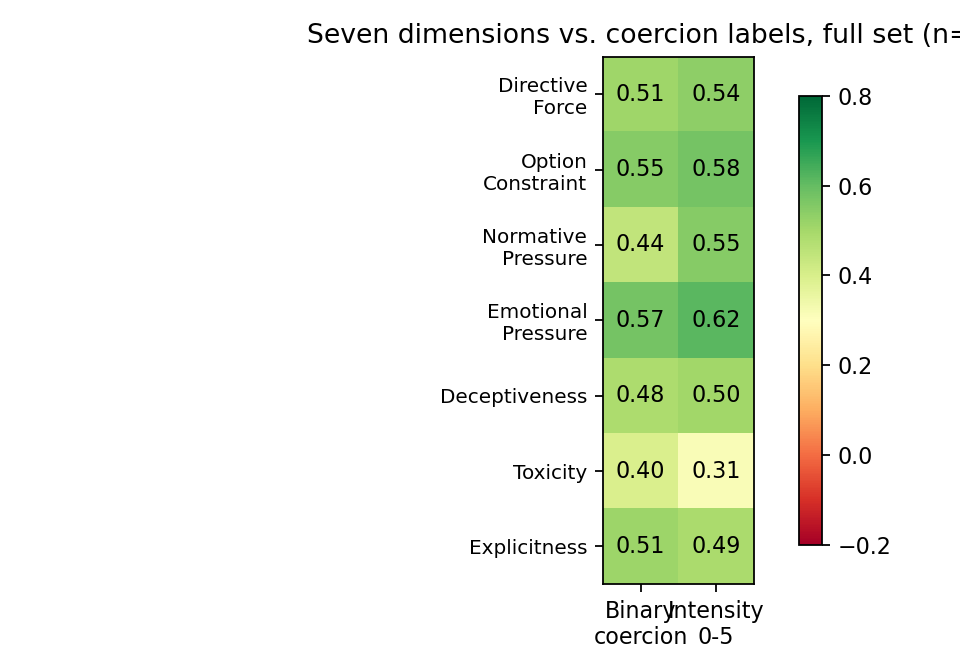
\includegraphics[width=0.70\linewidth]{figs/fig1_full_dims_vs_gold.png}
\caption{Seven dimensions versus the binary and 0--5 intensity labels on
the full release ($n{=}3{,}432$; Spearman correlation).}
\label{fig:dim-gold-full}
\end{figure}

\begin{figure}[t]
\centering
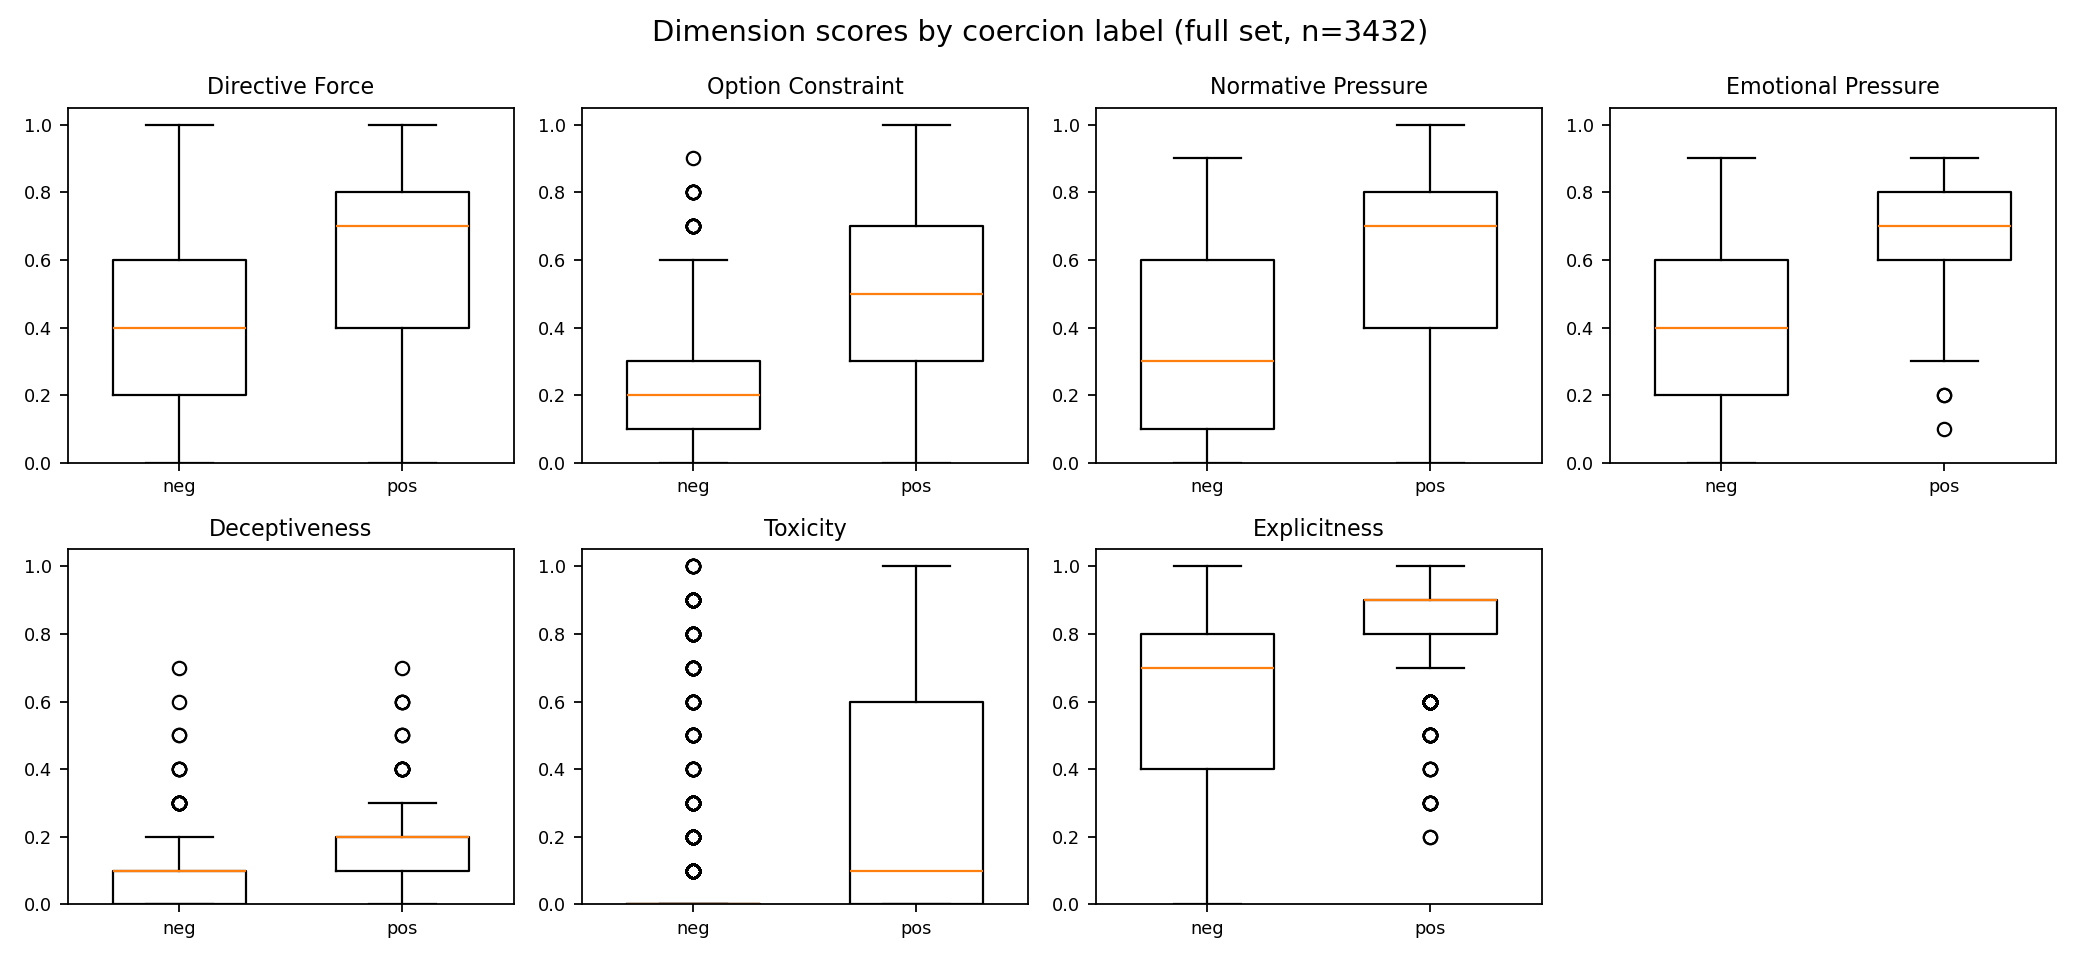
\includegraphics[width=0.70\linewidth]{figs/fig2_full_boxplot_by_label.png}
\caption{Dimension scores for coercive versus non-coercive dialogues on
the full release ($n{=}3{,}432$).}
\label{fig:box-full}
\end{figure}

\begin{figure}[t]
\centering
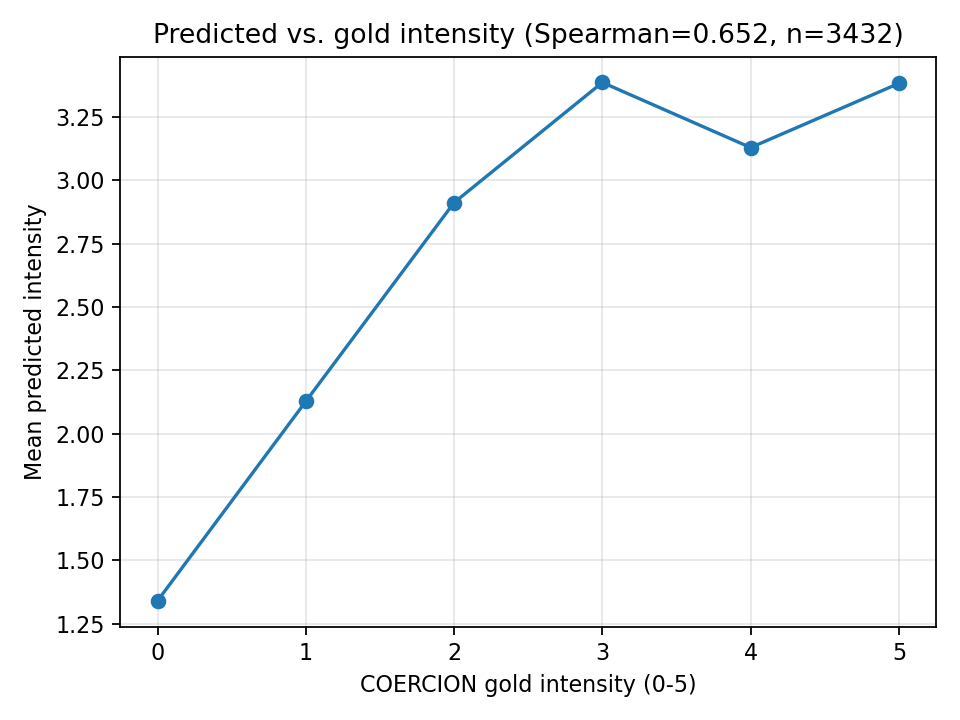
\includegraphics[width=0.70\linewidth]{figs/fig3_full_intensity_monotonic.png}
\caption{Predicted intensity as a function of the gold 0--5 intensity
label on the full release; points are within-level means.}
\label{fig:mono-full}
\end{figure}

\begin{figure}[t]
\centering
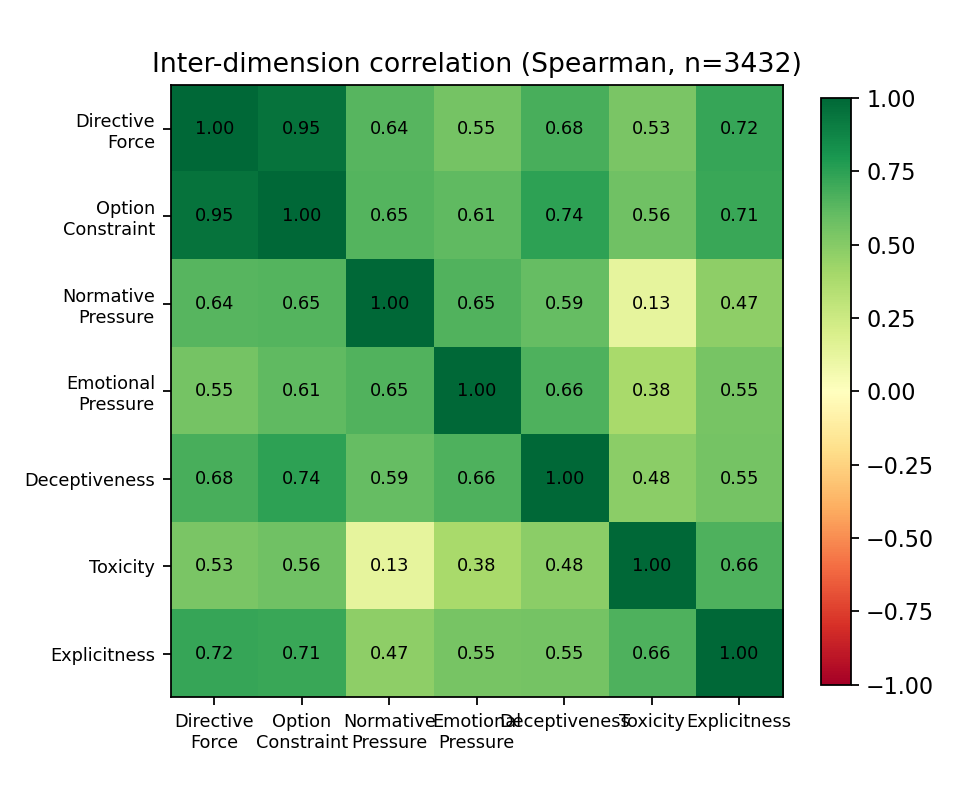
\includegraphics[width=0.70\linewidth]{figs/fig4_full_dim_corr.png}
\caption{Inter-dimension correlation matrix on the full release
(Spearman).}
\label{fig:dim-corr-full}
\end{figure}

\textbf{Ethics and data scope.} The dataset contains de-identified English
dialogues, and the release adds no new personal information or data
collection. Detailed provenance, human-subjects considerations, annotation
welfare, dual-use risk, cultural scope, and the accompanying datasheet are
provided in Appendix~\ref{app:ethics}.
\section{Experimental Design and Evaluation Protocol}
\label{sec:exp}
This section turns the conceptual claim into falsifiable tests. T1 asks
whether agentive force can be detected, T2 asks whether its strategies can be
recognized from the shared profile, and T3 asks whether the same profile
orders pressure by intensity. The ablations and cross-domain tests then
probe whether the representation is useful beyond the source corpus.
\subsection{Tasks}
\LNGF{} defines three tasks at increasing granularity.
\textbf{T1 (manipulation detection)} is a binary classification of whether a
dialogue exerts agentive force beyond the transparent baseline.
\textbf{T2 (type recognition)} is a fifteen-way multi-label classification
of the strategies in Table~\ref{tab:taxonomy}; type labels are released for
both the held-out split and the full release. \textbf{T3 (intensity
prediction)} is ordinal regression of the 0--5 intensity, evaluated with
quadratic weighted kappa (QWK) and accuracy-within-$\pm1$.

\subsection{Models and the Two-Stage Pipeline}
The pipeline is designed to isolate the proposed intermediate representation:
if a profile-based readout matches or improves a direct judge, the gain is
evidence that the dimensions expose decision-relevant structure rather than
merely renaming the final prediction.
Figure~\ref{fig:pipeline} shows the two-stage dimension-aware pipeline.
An upstream LLM parses a dialogue into an \emph{agentive profile}, the
seven-dimension vector at both turn and dialogue level; a downstream model
consumes the profile as structural anchors and predicts T1/T2/T3. This
two-stage design decouples dimension extraction from classification. We
compare three aggregation modes---turn-level only (T), global only (G), and
turn+global (B)---since aggregation granularity is known to affect
dimension-based classification.

\begin{figure*}[t]
\centering
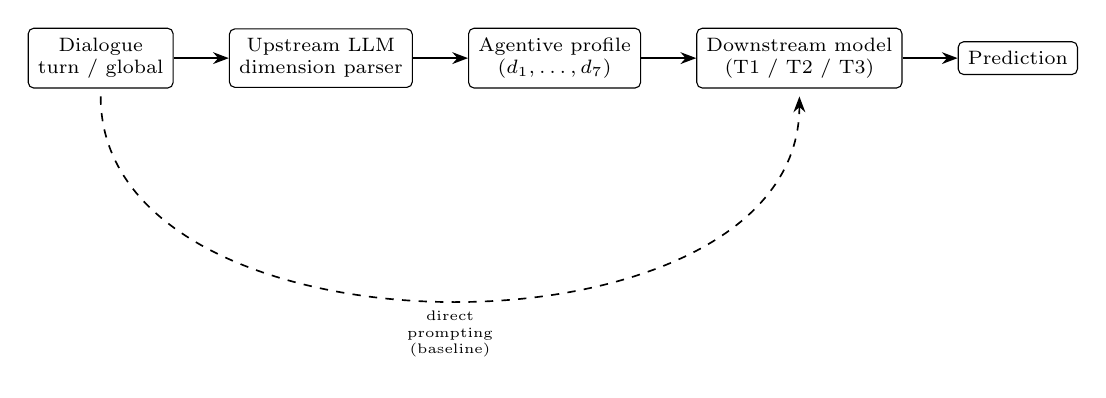
\begin{tikzpicture}[
  box/.style={draw, rounded corners=2pt, align=center, font=\scriptsize, inner sep=3.5pt},
  arr/.style={-{Stealth[length=2mm]}, semithick}
]

\node[box] (dlg) {Dialogue\\ turn / global};

\node[box, right=7mm of dlg] (up) {Upstream LLM\\ dimension parser};

\node[box, right=7mm of up] (prof) {Agentive profile\\ $(d_1,\dots,d_7)$};

\node[box, right=7mm of prof] (down) {Downstream model\\ (T1 / T2 / T3)};

\node[box, right=7mm of down] (out) {Prediction};
\draw[arr] (dlg) -- (up);
\draw[arr] (up) -- (prof);
\draw[arr] (prof) -- (down);
\draw[arr] (down) -- (out);
\draw[arr, dashed] ($(dlg.south)+(0,-1mm)$) to [out=-90,in=-90] node[midway, below, align=center, font=\tiny]{direct\\ prompting\\ (baseline)} ($(down.south)+(0,-1mm)$);
\end{tikzpicture}
\caption{Two-stage dimension-aware pipeline. The dashed path is the direct
prompting baseline used to isolate the effect of dimension anchoring.}
\label{fig:pipeline}
\end{figure*}

The pipeline is evaluated zero-shot: a frozen instruction-tuned LLM
(DeepSeek) parses each dialogue into the profile, and a direct judge that
skips the profile serves as control. Prompt variants include zero-shot,
chain-of-thought~\cite{wei2022}, and self-reflection, following the
self-perception approach of MultiManip~\cite{multimanip}
(Table~\ref{tab:models}).

\begin{table}[t]
\centering
\caption{Model configuration for the zero-shot evaluation in this release.}
\label{tab:models}
\footnotesize
\begin{tabular}{@{}lll@{}}
\toprule
\textbf{Model} & \textbf{Role} & \textbf{Tuning}\\
\midrule
DeepSeek & upstream dimension parser & frozen\\
DeepSeek & direct zero-shot judge & frozen\\
\bottomrule
\end{tabular}
\end{table}

\subsection{Experimental Setup}
The setup keeps the upstream parser frozen so that the reported comparisons
test representation and aggregation choices, not task-specific fine-tuning.
All evaluation is zero-shot: a frozen DeepSeek parses each dialogue into the
seven-dimension profile and a dialogue-level intensity at temperature~$0$;
T1 and T3 are read off the profile directly, with no fine-tuning. The control
is a direct zero-shot judge that skips the profile (dashed path in
Fig.~\ref{fig:pipeline}). Metrics are binary AUC and best F1 over the
intensity threshold for T1, and Spearman, QWK, and accuracy-within-$\pm1$
for T3. Cross-domain transfer uses the same frozen parser on four public
corpora.


\subsection{Research Questions}
The experiments are organized around four progressively stronger claims:
measurement consistency, complementary structure, transfer to related forms
of pressure, and robustness to implementation choices.
\textbf{RQ1 (annotation consistency):} Do the seven dimensions align with
the source pressure annotations? On the 634-dialogue and full 3{,}432-dialogue
releases (Sections~\ref{sec:firstrelease}--\ref{sec:fullscale}), report
per-dimension correlation with the source binary pressure label and 0--5 intensity
label, plus each dimension's AUC for separating coercive from non-coercive
dialogues.

\textbf{RQ2 (dimension structure):} Do the seven dimensions carry distinct,
complementary signal? Report per-dimension scores and AUCs, examine the
inter-dimension correlation matrix for expected couplings (e.g., $D_3$--$D_4$)
and unexpected ones (e.g., $D_5$--$D_6$), and analyze per-family profiles
(Section~\ref{sec:results}).

\textbf{RQ3 (zero-shot generalization):} Can dimension conditioning detect
unseen manipulation types? Cross-domain transfer to corpora whose types are
never seen during training (Section~\ref{sec:exp}) yields AUROC 0.742 on
MentalManip, 0.706 on MultiManip, and 0.729 on TalkDown. Within-taxonomy
leave-one-type-out shows a held-out type is not a separable novel cluster
(mean novelty AUROC 0.54, near chance), consistent with types being graded on
shared continuous dimensions rather than disjoint clusters. Crucially, the
pipeline still flags unseen types as manipulative: predicted intensity
separates any-strategy from benign dialogues with AUROC 0.963. The framework
thus transfers as a pressure signal, while assigning the specific type label
remains open.

\textbf{RQ4 (engineering conclusions):} How do aggregation mode and prompt
design interact with the pipeline? Using the same linear readout as
Table~\ref{tab:ablation} (train full release, held-out evaluation):
\emph{aggregation} (Table~\ref{tab:agg}) compares global-only (G),
turn-mean (T), and their concatenation (B). Turn-mean pooling collapses
toward chance (binary AUC 0.525) because pressure is concentrated in a
minority of turns and averaging dilutes it; B performs best (AUC 0.859,
Spearman 0.679, QWK 0.680). \emph{Prompt variants} (Table~\ref{tab:prompt})
are comparable (AUC 0.83--0.84), showing robustness to prompt design; CoT
marginally helps T1 and self-reflection T3. Remaining grid dimensions
(parser-model choice, ICC fidelity) are left to future work.

\begin{table}[t]
\centering
\caption{Aggregation ablation of the dimension-conditioned pipeline
(linear readout; train full release, held-out split). T mean-pools the
per-turn profiles over turns; B concatenates the turn-mean and global
profiles.}
\label{tab:agg}
\footnotesize
\begin{tabular}{@{}lccc@{}}
\toprule
\textbf{Aggregation} & \textbf{Binary AUC} & \textbf{Intensity $\rho$} & \textbf{QWK}\\
\midrule
G (global only) & 0.855 & 0.674 & 0.667\\
T (turn mean) & 0.525 & 0.040 & 0.066\\
B (turn+global) & \textbf{0.859} & \textbf{0.679} & \textbf{0.680}\\
\bottomrule
\end{tabular}
\end{table}

\begin{table}[t]
\centering
\caption{Prompt ablation of the upstream dimension parser (held-out
split, $n{=}634$). All variants use the same downstream linear readout.}
\label{tab:prompt}
\footnotesize
\begin{tabular}{@{}lccc@{}}
\toprule
\textbf{Prompt variant} & \textbf{T1 AUC} & \textbf{T3 Spearman} & \textbf{T3 QWK}\\
\midrule
Zero-shot & 0.832 & 0.666 & 0.623\\
Chain-of-thought & 0.839 & 0.639 & 0.613\\
Self-reflection & 0.838 & 0.670 & 0.630\\
\bottomrule
\end{tabular}
\end{table}

\subsection{Cross-Domain Evaluation}
This subsection tests the scope of the claim: a useful agentive-force profile
should transfer to related forms of listener-directed pressure, while
remaining distinguishable from toxicity that has no behavioral target.
To test transfer and distinctiveness, we evaluate the zero-shot pipeline on
existing resources with compatible labels: MentalManip~\cite{mentalmanip} and
MultiManip~\cite{multimanip} (psychological manipulation),
TalkDown~\cite{talkdown2023} (patronizing language), and
ToxicChat~\cite{toxicchat2023} (toxicity). We report each corpus's standard
metric under its own decision rule plus threshold-free AUROC, and use the
cross-corpus confusion to identify which constructs are shared with agency
and which are distinct. ReaMent~\cite{reament} and SemEval-2023
Task~3~\cite{piskorski2023} are left as future work.

\subsection{Dimension Contribution and Anchoring}
This subsection asks whether the dimensions carry complementary information
about agentive force. A strong result requires more than high aggregate
accuracy: removing a dimension should change performance in a way consistent
with its proposed mechanism, and a simple readout should retain the signal.
Each dimension's contribution is measured by consistency with the gold
labels (per-dimension Spearman and AUC, Table~\ref{tab:full}) and by a
marginal-contribution analysis: a linear readout over the seven scores
(logistic for binary, linear for intensity), trained on the full release and
evaluated on the held-out split, reaches binary AUC 0.855 and intensity
Spearman 0.674---slightly above the LLM's dimension-conditioned readout
(AUC 0.831, Spearman 0.665)---so the profiles carry the decision-relevant
signal without an LLM. Table~\ref{tab:ablation} reports leave-one-dimension-out
results: removing toxicity ($D_6$) degrades detection most (AUC drop 0.008)
and normative pressure ($D_3$) degrades intensity most (Spearman drop 0.021).
Notably, $D_6$ has the weakest univariate correlation yet its removal hurts
detection most, indicating non-redundant information (e.g., separating
hostile-but-non-coercive dialogues); $D_4$ is largely redundant with $D_3$,
and the remaining dimensions have small marginal effects, consistent with
Figure~\ref{fig:dim-corr-full}.



\begin{table}[t]
\centering
\caption{Leave-one-dimension-out ablation with a linear readout over the
seven dimension scores (held-out split, $n{=}634$). $\rho$: Spearman
correlation of predicted intensity with the gold 0--5 label. The LLM
readout is the dimension-conditioned zero-shot reference.}
\label{tab:ablation}
\footnotesize
\begin{tabular}{@{}lcc@{}}
\toprule
\textbf{Readout} & \textbf{Binary AUC} & \textbf{Intensity $\rho$}\\
\midrule
7-dim linear readout & 0.855 & 0.674\\
\;\;$-D_1$ (directive force) & 0.854 & 0.674\\
\;\;$-D_2$ (option constraint) & 0.851 & 0.668\\
\;\;$-D_3$ (normative pressure) & 0.851 & 0.653\\
\;\;$-D_4$ (emotional pressure) & 0.860 & 0.693\\
\;\;$-D_5$ (deceptiveness) & 0.855 & 0.674\\
\;\;$-D_6$ (toxicity) & 0.847 & 0.669\\
\;\;$-D_7$ (explicitness) & 0.853 & 0.674\\
\midrule
LLM readout (reference) & 0.831 & 0.665\\
\bottomrule
\end{tabular}
\end{table}

\subsection{Dimension-Space Structure}
\label{sec:viz}
This subsection tests whether the proposed dimensions organize strategy
families into interpretable pressure profiles rather than merely reproducing
one binary boundary. The expected result is partial overlap with distinct
mechanism-specific concentrations, since strategies can share dimensions.
To verify that the seven dimensions carve distinct, interpretable regions
for the four strategy families, Figure~\ref{fig:tsne} embeds the 3{,}432
dialogue profiles in two dimensions (t-SNE), colored by the dominant
family, together with the 226 dialogues for which no strategy was detected
(benign). Families occupy distinguishable regions, and benign dialogues
cluster at the low-pressure side. A logistic classifier over the seven raw
dimensions separates the five groups with 0.640 accuracy (chance 0.2) in
five-fold cross-validation, and each dimension alone separates benign from
manipulative dialogues with AUC 0.73--0.94. Figure~\ref{fig:famheat}
reports each family's mean dimension profile: the social-normative family
peaks on normative and emotional pressure ($D_3$, $D_4$), the exchange
family on option constraint and toxicity ($D_2$, $D_6$), the covert family
on emotional pressure ($D_4$), and benign dialogues are uniformly low
across all dimensions.

\begin{figure*}[t]
\centering
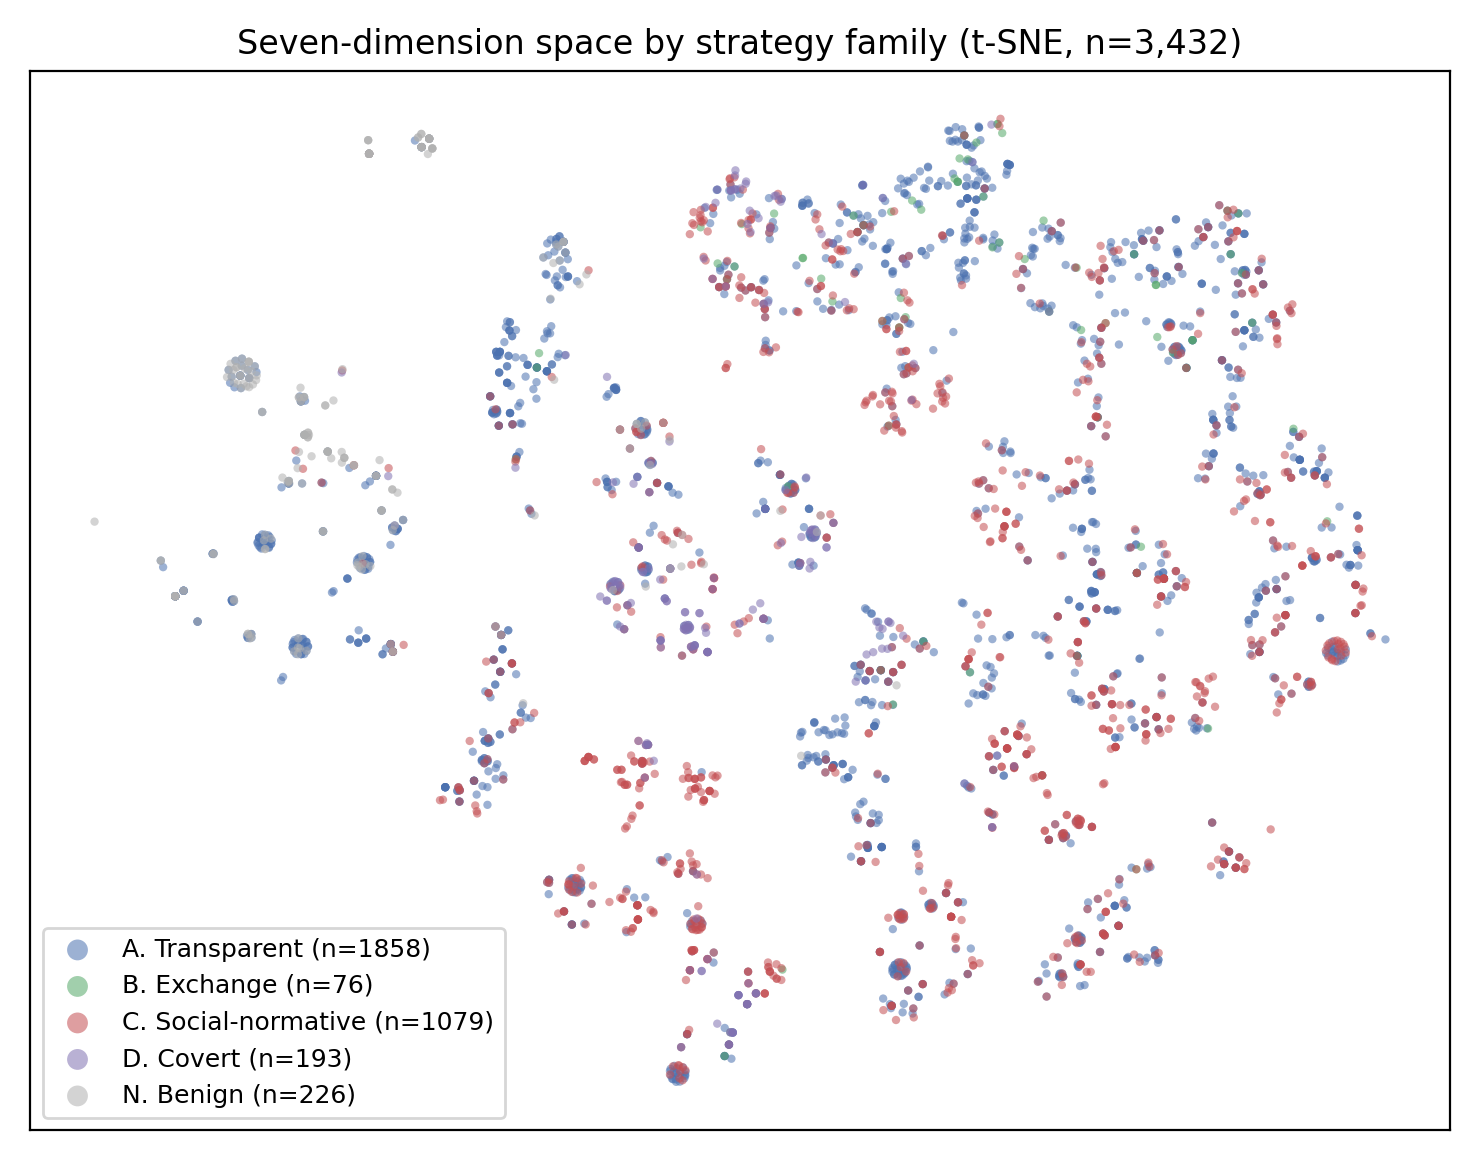
\includegraphics[width=0.50\textwidth]{figs/fig5_tsne_family.png}
\caption{t-SNE embedding of the seven-dimension profiles ($n{=}3{,}432$),
colored by dominant strategy family; the 226 no-strategy dialogues form the
benign group.}
\label{fig:tsne}
\end{figure*}

\begin{figure}[t]
\centering
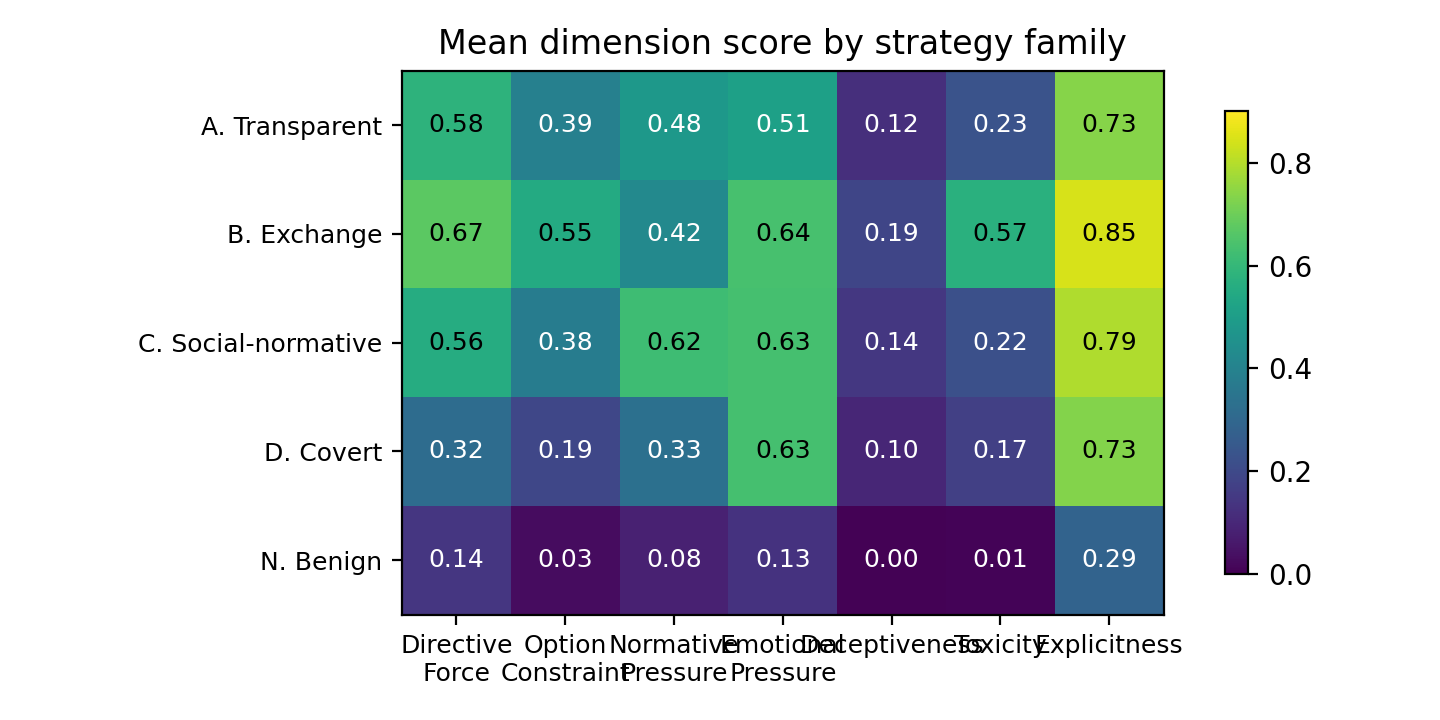
\includegraphics[width=0.85\linewidth]{figs/fig6_family_dims_heatmap.png}
\caption{Mean dimension score per strategy family. Social-normative and
covert families concentrate pressure on normative/emotional dimensions;
benign dialogues are uniformly low.}
\label{fig:famheat}
\end{figure}

\subsection{Results on the Full Release}
\label{sec:results}
This subsection brings the evidence together. It asks whether the profile
improves detection and intensity prediction over a holistic judgment, and
whether that improvement survives transfer and fine-grained type recognition.
Table~\ref{tab:results-t1} and Table~\ref{tab:results-t23} report the
zero-shot results of the dimension-conditioned pipeline on the full
3{,}432-dialogue release: a dialogue is decoded into the seven-dimension
profile (Section~\ref{sec:exp}), the profile is mapped to a 0--5 intensity,
and T1 and T3 are read off directly. As a control, Table~\ref{tab:results-t1}
also reports a direct zero-shot judge that skips the dimension profile
(dashed path in Fig.~\ref{fig:pipeline}) on the first-release split. The
dimension-conditioned readout reaches binary AUC 0.852 and best F1 0.817 on
the full release, exceeding the direct judge (AUC 0.780, best F1 0.755) and
the first-release estimate (AUC 0.832, F1 0.795); the fine-grained profile
therefore carries information that a single holistic judgment misses, and
the estimate is stable as the corpus grows. On the 0--5 intensity scale the
readout is well calibrated (QWK 0.595, Spearman 0.651, accuracy within
$\pm1$ of 0.692 on the full release), with only a modest drop from the
first-release values as hard negatives and the intensity tail are added.

The cross-domain transfer results (Table~\ref{tab:results-x}) support the
interpretability and discriminative-validity claims. Under a threshold-free
ranking, the zero-shot judge transfers moderately to the psychological-
manipulation corpora (AUROC 0.742 on MentalManip, 0.706 on MultiManip) and to
patronizing language (AUROC 0.729 on TalkDown), while transfer to generic
toxicity is weak (AUROC 0.587 on ToxicChat). This pattern is consistent with
the design: manipulation and condescension exert listener-directed pressure
and are therefore partially captured by the agency dimensions, whereas
generic toxicity is largely distinct from agency. Fixed-threshold
macro-F1/F1 values are much lower (e.g., 0.058 on TalkDown) because the
intensity scale is calibrated on our annotation scheme and the judge rarely
assigns intensity $\ge$3 to dialogues annotated under other corpora's
schemes: ranking (AUROC) transfers, absolute calibration does not.
Target-calibrated thresholds recover macro-F1 around 0.68--0.74 on the
manipulation corpora.
 T2 type recognition is evaluated with a lightweight one-vs-rest logistic
readout over the seven dimension scores, contrasted with a supervised
baseline that fine-tunes RoBERTa-base end-to-end on the dialogue text
(Table~\ref{tab:rq2}). We report two protocols for the readout. First, it
is trained on the full 3{,}432-dialogue release and evaluated on the
type-labeled held-out split: family-level recognition reaches micro-F1 0.827
and macro-F1 0.772, and type-level recognition reaches micro-F1 0.668 and
macro-F1 0.480. Five-fold cross-validation over the full release yields
similar estimates (family micro-F1 0.820 and macro-F1 0.752; type micro-F1
0.669 and macro-F1 0.477), so the results are stable as the corpus grows
from 634 to 3{,}432 dialogues. The fine-tuned RoBERTa baseline gives
consistent cross-validation estimates as well (type macro-F1 0.540, micro-F1
0.734; family macro-F1 0.767, micro-F1 0.815), confirming that the held-out
results are not sensitive to the train/test split. The fine-tuned
RoBERTa-base is clearly
stronger at type level (macro-F1 0.544, micro-F1 0.731 on the held-out
split), confirming that the type labels are learnable by a supervised model;
at family level it matches the readout (macro-F1 0.780, micro-F1 0.820), so
the dimension readout remains a competitive lightweight and interpretable
baseline. Type-level macro-F1 is depressed by three rare types (rational
persuasion $A_3$, authority $C_4$, deception/gaslighting $D_2$), which
appear in fewer than thirty of the 3{,}432 dialogues; family-level results
are the more reliable target for this corpus, and the full type labels are
released for downstream use.

\begin{table}[t]
\centering
\caption{T2 type recognition: a one-vs-rest logistic readout over the seven
dimension scores versus fine-tuned RoBERTa-base. ``Held-out'': trained on
the full release ($n{=}3{,}432$), evaluated on the type-labeled held-out
split ($n{=}634$); ``5-fold CV'': cross-validation over the full release.
F1 is macro/micro at the best threshold.}
\label{tab:rq2}
\footnotesize
\begin{tabular}{@{}lcccc@{}}
\toprule
& & \multicolumn{2}{c}{Linear readout} & \multicolumn{1}{c}{RoBERTa-base}\\
\cmidrule(lr){3-4}\cmidrule(lr){5-5}
\textbf{Granularity} & \textbf{Protocol} & Macro-F1 & Micro-F1 & Macro/Micro-F1\\
\midrule
15 types & Held-out & 0.480 & 0.668 & 0.544 / 0.731\\
15 types & 5-fold CV & 0.477 & 0.669 & 0.540 / 0.734\\
4 families & Held-out & 0.772 & 0.827 & 0.780 / 0.820\\
4 families & 5-fold CV & 0.752 & 0.820 & 0.767 / 0.815\\
\bottomrule
\end{tabular}
\end{table}

\begin{table}[t]
\centering
\caption{T1 detection on the full release ($n{=}3{,}432$): the
dimension-conditioned readout, versus the same readout on the first-release
split ($n{=}634$) and a direct zero-shot judge that skips the profile
(dashed path in Fig.~\ref{fig:pipeline}). ``Best F1'' is the maximum F1
over the intensity threshold.}
\label{tab:results-t1}
\footnotesize
\begin{tabular}{@{}lccc@{}}
\toprule
\textbf{Metric} & \textbf{Full} & \textbf{First} & \textbf{Direct}\\
 & ($n{=}3{,}432$) & \textbf{release} & \textbf{zero-shot}\\
\midrule
Binary AUC & 0.852 & 0.831 & 0.780\\
Best F1 (threshold) & 0.817 (3) & 0.795 (3) & 0.755 (3)\\
Accuracy @ best F1 & 0.789 & 0.760 & 0.711\\
\midrule
Best per-dimension AUC ($D_2$) & 0.829 & 0.825 & ---\\
\bottomrule
\end{tabular}
\end{table}

\begin{table}[t]
\centering
\caption{T3 intensity prediction from the dimension-conditioned pipeline on
the full release ($n{=}3{,}432$), with the first-release ($n{=}634$) values
for comparison.}
\label{tab:results-t23}
\footnotesize
\begin{tabular}{@{}lcc@{}}
\toprule
\textbf{Metric} & \textbf{Full} & \textbf{First release}\\
\midrule
Spearman $\rho$ & 0.651 & 0.665\\
Pearson $r$ & 0.677 & 0.691\\
Quadratic weighted kappa & 0.595 & 0.623\\
Accuracy within $\pm 1$ & 0.692 & 0.722\\
Exact match & 0.216 & 0.219\\
\bottomrule
\end{tabular}
\end{table}

\begin{table}[t]
\centering
\caption{Cross-domain zero-shot transfer of the seven-dimension pipeline.
``Standard metric'' is each corpus's own metric under the source-task
decision rule (intensity ${\ge}3$); ``AUROC'' is threshold-free and directly
comparable. Sampled subsets: MentalManip $n{=}300$, MultiManip $n{=}220$,
TalkDown $n{=}652$, ToxicChat $n{=}300$.}
\label{tab:results-x}
\footnotesize
\begin{tabular}{@{}lccc@{}}
\toprule
\textbf{Corpus} & \textbf{Standard metric} & \textbf{Zero-shot} & \textbf{AUROC}\\
\midrule
MentalManip & macro-F1 & 0.615 & 0.742\\
MultiManip & macro-F1 & 0.347 & 0.706\\
TalkDown & F1 & 0.058 & 0.729\\
ToxicChat & AUROC & 0.587 & 0.587\\
\bottomrule
\end{tabular}
\end{table}


\subsection{Limitations and Threats to Validity}
Several limitations should be acknowledged. First, the seven dimensions are
a design choice; a finer or coarser decomposition is possible. We mitigate
this by reporting consistency against the source pressure labels at both
first-release and full-scale level. Second, cross-platform variation in
norms and politeness may limit transferability; the cross-domain evaluation
and a planned cross-lingual extension bound this risk. Third, annotation of
covert strategies such as gaslighting is inherently subjective; our
two-annotator study (Section~\ref{sec:qc}) shows deceptiveness ($D_5$) is
the least reliable dimension, which we report rather than hide. Fourth, the
dataset inherits the sampling biases of the source corpus, documented in the
data statement. Finally, the benchmark measures the \emph{exertion} of
agentive force, not its \emph{effect}: a coercive dialogue the listener
resists is still annotated as high-pressure, correct for detection but not
evidence of harm. This is a resource and analysis benchmark rather than a
claim of a complete theory of coercion; the seven dimensions are meant to
be a practical, falsifiable abstraction that future datasets can refine.


\subsection{Discussion}
Three outcomes matter beyond the numbers. First, reliable dimension profiles
provide a continuous, interpretable measurement of how language exerts
pressure---from transparent requests to covert manipulation under one
rubric---and locate each strategy family precisely in this space. Second,
distinct per-family profiles let system designers select parsers and
aggregation modes from a small set of validated configurations rather than
re-tuning per task. Third, the profile offers an interpretable audit trail:
a detection system can justify a ``coercive'' verdict with concrete dimension
evidence (e.g., high $D_3$, low $D_7$), the accountability that binary
toxicity scores cannot provide. These implications motivate releasing the
gold dimension profiles and parser outputs with the benchmark. The central
payoff is a shared intermediate representation that makes comparison,
auditing, and error analysis possible across different kinds of pressure.


\section{Conclusion}
We presented \LNGF{}, a new dataset and unified benchmark for the \afd{} in
real-world multi-turn dialogues. The full release contains 3{,}432 dialogues
annotated with dialogue-level intensity and seven universal psychological
dimensions, and its reliability is verified through consistency with the
source pressure labels. We further specify three benchmark tasks, a
two-stage dimension-aware pipeline, and research questions on dimension
structure and zero-shot generalization. A zero-shot dimension-conditioned
readout reaches binary AUC 0.852 and best F1 0.817 on the full release,
exceeding a direct zero-shot judge, and transfers moderately to
psychological-manipulation and patronizing-language corpora while remaining
distinct from generic toxicity. Future work includes stronger multi-parser
evaluation, cross-lingual extension, and studying how agentive force
interacts with listener vulnerability and cultural norms.

\appendices
\section{Ethics and Privacy}
\label{app:ethics}
The dialogues are de-identified and this work performs re-annotation rather
than new collection. The release adds no personal information. The study
does not collect behavioral or demographic data; the manual checks use
already-anonymized text. Annotators may skip distressing content and take
breaks. Because the taxonomy could be misused to craft manipulative language,
the release is intended for research on detection and analysis, not automated
moderation, surveillance, or consequential decisions without human review.
The current data are English and drawn from everyday scenarios, so cultural
and cross-lingual validity remains an open question. A datasheet documents
composition, preprocessing, intended uses, and limitations.

{\small
\setlength{\itemsep}{1pt}\setlength{\parsep}{0pt}
\bibliographystyle{IEEEtran}
\bibliography{references,references_extra}
}

\end{document}
